\documentclass[10pt,a4paper]{article}

\usepackage[utf8]{inputenc}
\usepackage[english]{babel}
\usepackage[T1]{fontenc}
\usepackage{amsmath}
\usepackage{amsfonts}
\usepackage{amssymb}
\usepackage{graphicx}
\usepackage{lmodern}
\usepackage{hyperref}
\usepackage[left=2.7cm,right=2.7cm,top=2cm,bottom=3cm]{geometry}
\usepackage{verbatim}
\usepackage{xcolor}
\usepackage{url}

\hypersetup{
    colorlinks,
    linkcolor={red!50!black},
    citecolor={blue!50!black},
    urlcolor={blue!80!black}
}

\title{
\includegraphics[scale=1]{Art/otb-logo.png}\\
  OTB Installation Guide\\
  Updated for OTB-5.10.1\\
  {\small\url{https://www.orfeo-toolbox.org}}
}

\begin{document}

\maketitle

\tableofcontents

\clearpage

\section{Windows}

\subsection{QGIS}
Install QGIS: \url{http://www.qgis.org/en/site/forusers/download.html}.

\subsection{OTB and Monteverdi}

To install OTB and Monteverdi, download the appropriate package for your
architecture (32 or 64 bits). If you have a 32 bit machine:

\begin{verbatim}
Download OTB-5.10.1-xdk-win32.zip
\end{verbatim}

If you have a 64 bit machine:

\begin{verbatim}
Download OTB-5.10.1-xdk-win64.zip
\end{verbatim}

These files are available at:
\url{https://orfeo-toolbox.org/packages/xdk/}.

Extract the zip archive in your personal folder, for instance in:\\
\begin{centering}
\texttt{C:{\textbackslash}projects}.
\end{centering}

You can of course use an other directory. The next step is to update PATH
environment variable. This must be done one time before starting using OTB package.

\begin{verbatim}
open cmd.exe (DOS command)
cd C:\projects\OTB-5.10.1-xdk-win64
set PATH=C:\projects\OTB-5.10.1-xdk-win64\bin;%PATH%
\end{verbatim}

\subsection{Test the installation}
Once the installation is done, OTB applications can be used in several
ways. Check that you have a working OTB with the following steps:

\begin{enumerate}

\item Launch \texttt{monteverdi.bat} from the installation folder.

\item Try to open a tif image in Monteverdi (see
figure~\ref{fig:monteverdi}). A demonstration tif image is available here: \url{https://git.orfeo-toolbox.org/otb-data.git/blob/HEAD:/Examples/QB\_Toulouse\_Ortho\_PAN.tif}.

\item The application browser is available from the ``View'' menu 
$\rightarrow$ "OTB-Applications browser".
(see figure \ref{fig:windows-mapla}).

\item Go to the \texttt{bin} folder in the OTB install directory and double-click on the \texttt{.bat} file corresponding to the application to be run, for instance:\\
\texttt{John{\textbackslash}install{\textbackslash}OTB-5.10.1-win32{\textbackslash}bin{\textbackslash}otbgui\_Rescale.bat}
(see figure \ref{fig:windows-otbgui}).

\end{enumerate}

\begin{figure}[!htbp]
  \center
  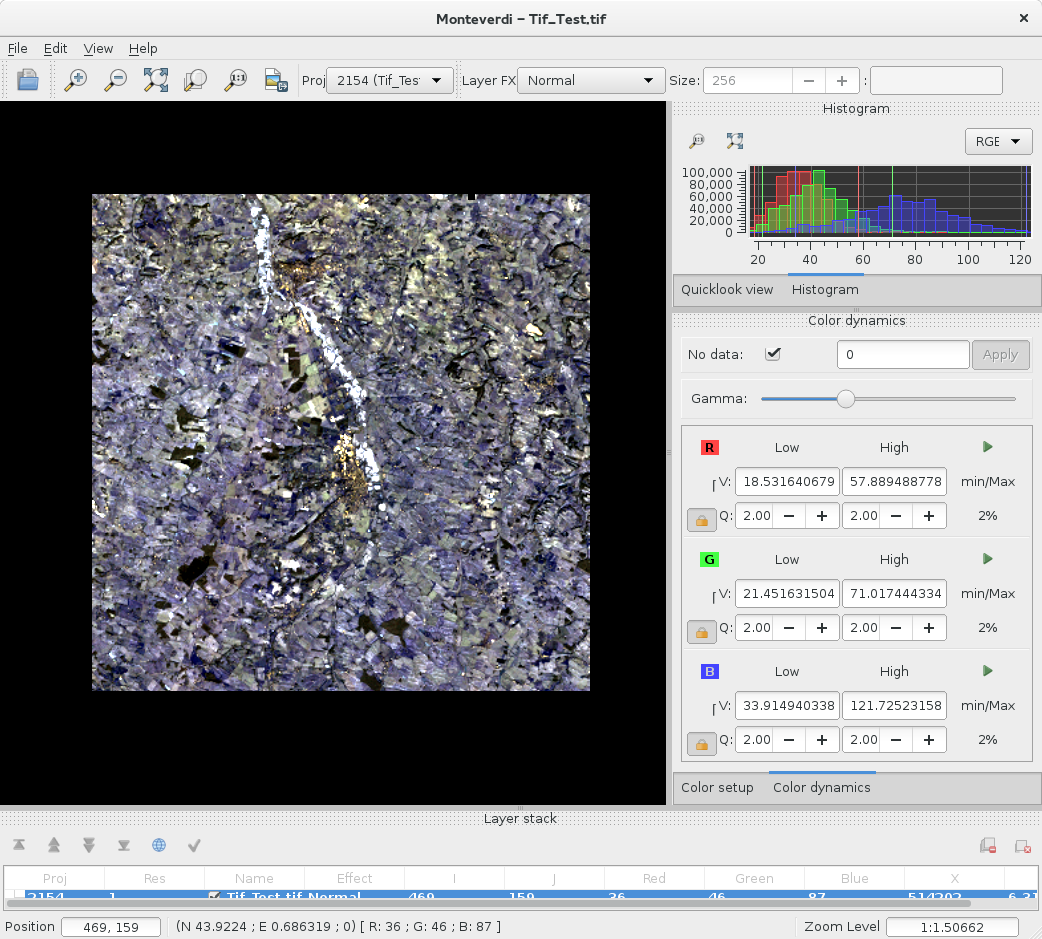
\includegraphics[width=0.7\textwidth]{Art/monteverdi-tif.png}
  \caption[]{Monteverdi}
  \label{fig:monteverdi}
\end{figure}

\begin{figure}[!htbp]
  \center
  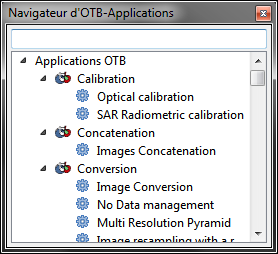
\includegraphics[width=0.7\textwidth]{Art/windows-mapla.png}
  \caption[]{OTB applications can be used from Monteverdi}
  \label{fig:windows-mapla}
\end{figure}

\begin{figure}[!htbp]
  \center
  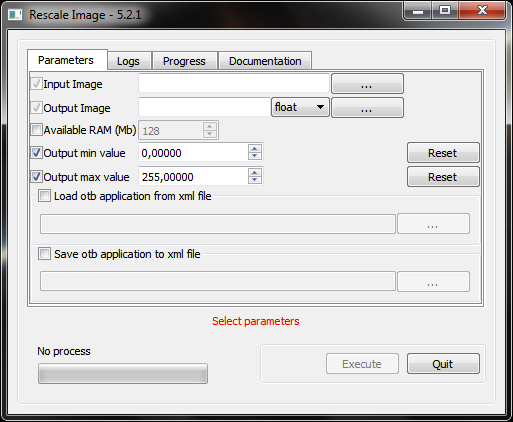
\includegraphics[width=0.7\textwidth]{Art/windows-otbgui.png}
  \caption[]{OTB Graphical User Interface}
  \label{fig:windows-otbgui}
\end{figure}


\subsection{Develop with OTB (only for participants of the developer session)}

This section describes how to set up the environment to develop in C++ on
Windows using OTB.
You have two methods to build your projects:
\begin{enumerate}
\item Using windows command prompt (cmd.exe)
\item Visual studio IDE
\end{enumerate}

You need Visual Studio 2015 and CMake for building projects using OTB.

\subsubsection{Clink (optional)}
Clink add Bash's powerful command line editing in
cmd.exe. The tool can be downloaded free of charge from their GitHub
page \url{https://github.com/mridgers/clink}. This tool is optional for both development and usage of OTB.
But it is highly recommended to use it rather than using third party terminal emulator such as git bash or
mobxterm.

\subsubsection{Visual Studio 2015}
Visual Studio Community Edition can be downloaded free of charge. However, you must register
to get access to the download page. We use community edition because it is free
of charge. If you have professional or enterprise edition that will work
too. The latest version is 2017 but you must have \textbf{Visual Studio 2015 for OTB}. 

Download visual studio 2015 from \url{https://www.visualstudio.com/vs/older-downloads/}

\subsubsection{CMake}
CMake installer for Windows can be downloaded from \url{https://cmake.org/files/v3.7/cmake-3.7.2-win64-x64.msi}
\newline
Make sure you add CMake to system PATH ((see figure \ref{fig:cmake-install}).

\begin{figure}[!htbp]
  \center
  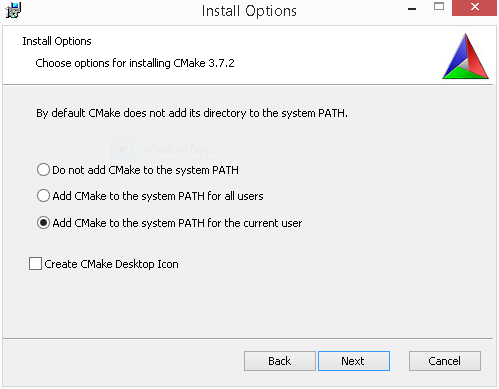
\includegraphics[width=0.7\textwidth]{Art/cmake-install.png}
  \caption[]{cmake-install}
  \label{fig:cmake-install}
\end{figure}

\textbf{CMake is not a required if you are building using the IDE (see section~\ref{ide}).}

\subsubsection{Develop using windows command prompt}
I've extracted xdk package into \texttt{C:{\textbackslash}projects}. So I will
update variables relative to this path.

\begin{itemize}
  \item Open cmd.exe
  \item The first step is to call \textbf{vcvarsall.bat} from Visual Studio 2015:
  \begin{verbatim}
    call "C:\Program Files (x86)\Microsoft Visual Studio 14.0\VC\vcvarsall.bat" x64
  \end{verbatim}
  \textbf{We assume you had installed visual studio to C: drive} \\
  \textbf{x64 is the machine architecture. For some systems, it is called amd64 or
  x86\_64.}
  \item The next step is to update PATH and CMAKE\_PREFIX\_PATH variables. PATH variable
is required for finding dll files. CMAKE\_PREFIX\_PATH variable is required for
finding packages with cmake configure:
\begin{verbatim}
set PATH=C:\projects\OTB-5.10.1-xdk-win64\bin;$PATH
set CMAKE_PREFIX_PATH=C:/projects/OTB-5.10.1-xdk-win64
\end{verbatim}

\end{itemize}
  
\subsubsection{Configure and build project}

We can try to build a simple program using cmake to test the configuration:

\begin{verbatim}
cd c:\projects\otbprojects\build
cmake ..\ex1_HelloWorld -G"NMake Makefiles"
nmake
\end{verbatim}
If build goes fine, you will get executable file HelloWorld.exe
\newline
C:{\textbackslash}projects{\textbackslash}otbprojects{\textbackslash}build{\textbackslash}HelloWorld.exe
\newline

\subsubsection{Test the Hello World program}

The last step is to run the generated executable:

\begin{verbatim}
> c:\projects\otbprojects\build\HelloWorld.exe
> OTB Hello World !
\end{verbatim}

\subsubsection{Using Visual Studio IDE}\label{ide}

Please see the wiki page which describes how to set up visual studio project to
develop with OTB:
\url{https://wiki.orfeo-toolbox.org/index.php/Writing_OTB_modules_with_Visual_Studio_IDE}

\clearpage
\section{Linux (Ubuntu example)}


\subsection{QGIS}
QGIS can be installed via a command line like:
\begin{verbatim}
sudo apt-get install qgis
\end{verbatim}

\subsection{Dependencies installation}
Before installing the self-extracting Linux binary for OTB, several system dependencies have to be installed. In a terminal, type the following:
\begin{verbatim}
sudo apt-get install libx11-6 libxext6 libxau6 libxxf86vm1 libxdmcp6 libdrm2
\end{verbatim}
or the equivalent for other distributions.

You will need the libgl1 and libglu1 libraries, which have different implementations (MESA, FGLRX, NVIDIA, etc.). If you don't already have these libraries, you can use the MESA implementation:
\begin{verbatim}
sudo apt-get install libgl1-mesa-glx libglu1-mesa
\end{verbatim}

\subsection{Install OTB and Monteverdi}
Download the self-extracting binary for Linux (64 bits), available at:
\begin{center}
\url{https://orfeo-toolbox.org/packages/xdk/OTB-5.10/}
\end{center}

The self-extracting binary will extract itself in the current directory. First, the archive has to be made executable, and then it can be run:
\begin{verbatim}
chmod +x OTB-5.10.1-Linux64.run
./OTB-5.10.1-Linux64.run
\end{verbatim}

The executable binaries will be inside the 'bin' directory, and you can put this directory in your PATH variable if you want to. 

There are also scripts which set all the environment variables to allow to run Monteverdi and Mapla:
\begin{verbatim}
cd OTB-5.10.1-Linux64
. ./otbenv.profile
./monteverdi.sh
./mapla.sh
\end{verbatim}

\subsection{Test the installation}
Once the installation is done, OTB applications can be run in several ways. Check that you have a working installation with the following steps:
\begin{enumerate}

\item Try to open a tif image in Monteverdi (see
figure~\ref{fig:monteverdi}). A demonstration tif image is available here: \url{https://git.orfeo-toolbox.org/otb-data.git/blob/HEAD:/Examples/QB\_Toulouse\_Ortho\_PAN.tif}.

\item The application browser is available from the ``View'' menu 
$\rightarrow$ "OTB-Applications browser".
(see figure \ref{fig:windows-mapla}).

\item Run an application using the terminal, for instance
\texttt{otbgui\_Rescale}. (see figure \ref{fig:windows-otbgui}).

\end{enumerate}

\subsection{Develop with OTB (only for participants of the developer session)}

Make sure cmake and gcc (>= 4.9) are installed on your system. You can print
cmake and gcc versions with the following commands: 

\begin{verbatim}
cmake --version
gcc --version
\end{verbatim}

\subsubsection{Configure and build project}

\begin{verbatim}
cd ~/otbprojects/HelloWorld/
mkdir build
cmake ~/otbprojects/HelloWorld/ex1_HelloWorld -DCMAKE_CXX_FLAGS='-std=c++11'
make
\end{verbatim}

You now have \textasciitilde/otbprojects/HelloWorld/build/HelloWorld

\subsubsection{Test the Hello World program}

\begin{verbatim}
> ~/otbprojects/HelloWorld/build/HelloWorld
> OTB Hello World !
\end{verbatim}

\section{Mac OS X}

\subsection{QGIS}
Install QGIS: \url{http://www.qgis.org/en/site/forusers/download.html}.

\subsection{OTB and Monteverdi}

To install OTB and Monteverdi, download the appropriate package from \url{https://www.orfeo-toolbox.org/packages/xdk/OTB-5.10/}.

\begin{verbatim}
https://www.orfeo-toolbox.org/packages/xdk/OTB-5.10/OTB-5.10.1-xdk-Darwin64.run
\end{verbatim}

The self-extracting binary will extract itself in the current directory. First,
the archive has to be made executable, and then it can be run:

\begin{verbatim}
chmod +x OTB-5.10.1-xdk-Darwin64.run
./OTB-5.10.1-xdk-Darwin64
cd OTB-5.10.1-xdk-Darwin64
. ./otbenv.profile
\end{verbatim}

The installation is finished. You now have OTB-5.10.1-xdk-Darwin64 in your
directory.

\subsection{Test the installation}

\begin{enumerate}
\item OTB Applications: You can run OTB applications through otbgui\_<APPLICATION> and or otbcli\_<APPLICATION> 
\item Monteverdi : Start monteverdi using Monteverdi.app in OTB-5.10.1-xdk-Darwin64
\item Mapla : Start Mapla using Mapla.app in OTB-5.10.1-xdk-Darwin64
\end{enumerate}
It is advised not to run bin/monteverdi or bin/mapla directly (use .app files instead).

\subsection{Develop with OTB (only for participants of the developer session)}
Make sure cmake, and XCode (>= 6.1.1) are installed on your system. AppleClang
is installed with XCode.

Check cmake and gcc version with:

\begin{verbatim}
cmake --version
gcc --version
\end{verbatim}

\subsubsection{Configure and build project}

\begin{verbatim}
cd ~/otbprojects/HelloWorld/
mkdir build
cmake ~/otbprojects/HelloWorld/ex1_HelloWorld -DCMAKE_CXX_FLAGS='-std=c++11'
make
\end{verbatim}

You now have ~/otbprojects/HelloWorld/build/HelloWorld

\subsubsection{Test the Hello World program}

\begin{verbatim}
> ~/otbprojects/HelloWorld/build/HelloWorld
> OTB Hello World !
\end{verbatim}

\end{document}
